% *********************************************************************
% © 2021 Jeremy Sylvestre
%
% Permission is granted to copy, distribute and/or modify this document
% under the terms of the GNU Free Documentation License, Version 1.3 or
% any later version published by the Free Software Foundation; with no
% Invariant Sections, no Front-Cover Texts, and no Back-Cover Texts. A
% copy of the license is included in the appendix entitled “GNU Free
% Documentation License” that appears in the output document of this
% PreTeXt source code. All trademarks™ are the registered® marks of
% their respective owners.
%
% *********************************************************************

\newcommand*{\xmin}{-1}
\newcommand*{\xmax}{16}
\newcommand*{\ymin}{-0.5}
\newcommand*{\ymax}{3.5}

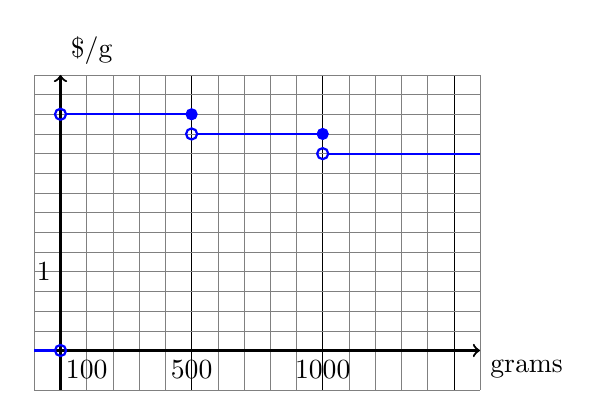
\begin{tikzpicture}
[
	closedpt/.style={circle,draw,fill,inner sep=0pt,minimum size=4pt},
	openpt/.style={circle,draw,inner sep=0pt,minimum size=4pt},
	xscale=0.333
]

	% grid
	\foreach \x in {-1,0,1,...,16} {
		\draw[very thin,gray] (\x,\ymin) -- (\x,\ymax);
	}
	\foreach \x in {5,10,15} {
		\draw[very thin,black] (\x,\ymin) -- (\x,\ymax);
	}
	\foreach \y in {-0.5,0,0.25,...,3.5} {
		\draw[very thin,gray] (\xmin,\y) -- (\xmax,\y);
	}

	% label grid
	\foreach \x in {1,5,10} {
		\node[below] at (\x,0) {${\x}00$};
	}
	\node[left] at (0,1) {$1$};

	% axes
	\draw[->,thick] (\xmin,0) -- (\xmax,0) node[below right] {grams};
	\draw[->,thick] (0,\ymin) -- (0,\ymax) node[above right] {$\$/\mathrm{g}$};

	% zero out negative amounts
	\node[blue,thick,openpt] at (0,0) (stop) {};
	\draw[blue,thick] (\xmin,0) -- (stop);

	% first step
	\node[blue,thick,openpt] at (0,3) (start) {};
	\node[blue,closedpt] at (5,3) (stop) {};
	\draw[blue,thick] (start) -- (stop);

	% second step
	\node[blue,thick,openpt] at (5,2.75) (start) {};
	\node[blue,closedpt] at (10,2.75) (stop) {};
	\draw[blue,thick] (start) -- (stop);

	% final step
	\node[blue,thick,openpt] at (10,2.5) (start) {};
	\draw[blue,thick] (start) -- (\xmax,2.5);

\end{tikzpicture}
